% =====================================================================
%  KMITL Thesis Defense Slides — Thai YouTube Virality Prediction
%  ผู้นำเสนอ: นายตรัยภูรินท์ สืบสุวรรณสาร (65050330)
%             นายธีรนนท์ ไชยลังกา      (65050417)
%             นายภาณุเดช ภู่โทสนธิ์     (65050685)
%  อาจารย์ที่ปรึกษา: ผศ. ดร. พรพิมล ชัยวุฒิศักดิ์
%  ระยะเวลา: 60 นาที (~50 นาทีนำเสนอ + 10 นาที Q&A)
%  คอมไพล์ด้วย: xelatex slides.tex (รัน 2 ครั้ง สำหรับ TOC)
% =====================================================================
\documentclass[aspectratio=169,11pt,xcolor=dvipsnames]{beamer}

% ── Thai/English fonts ────────────────────────────────────────────────
\usepackage{polyglossia}
\setdefaultlanguage{thai}
\setotherlanguage{english}
\usepackage{fontspec}
\defaultfontfeatures{Ligatures=TeX,Renderer=HarfBuzz}
\setmainfont[Path=fonts/,
  Extension=.ttf,
  UprightFont=THSarabunNew,
  BoldFont=THSarabunNew-Bold,
  ItalicFont=THSarabunNew-Italic,
  BoldItalicFont=THSarabunNew-BoldItalic,
  Scale=1.2]{THSarabunNew}
\setsansfont[Path=fonts/,
  Extension=.ttf,
  UprightFont=THSarabunNew,
  BoldFont=THSarabunNew-Bold,
  ItalicFont=THSarabunNew-Italic,
  BoldItalicFont=THSarabunNew-BoldItalic,
  Scale=1.2]{THSarabunNew}
\newfontfamily\thaifont[Path=fonts/,Extension=.ttf,
  UprightFont=THSarabunNew,BoldFont=THSarabunNew-Bold,Scale=1.2]{THSarabunNew}
% Thai monospace (polyglossia ต้องการ \thaifonttt — ใช้ TH Sarabun เพราะ
% Latin Modern Mono ไม่รองรับ Thai script)
\setmonofont[Path=fonts/,Extension=.ttf,
  UprightFont=THSarabunNew,BoldFont=THSarabunNew-Bold,Scale=1.0]{THSarabunNew}
\newfontfamily\thaifonttt[Path=fonts/,Extension=.ttf,
  UprightFont=THSarabunNew,BoldFont=THSarabunNew-Bold,Scale=1.0]{THSarabunNew}

% ── Packages ──────────────────────────────────────────────────────────
\usepackage{amsmath,amssymb}
\usepackage{booktabs,array,multirow}
\usepackage{graphicx}
\usepackage{tikz}
\usetikzlibrary{shapes.geometric,arrows.meta,positioning,fit,backgrounds,calc}
\usepackage{pgfplots}\pgfplotsset{compat=1.18}
\usepackage{xcolor}
\usepackage{listings}
\usepackage{caption}
\captionsetup[figure]{labelformat=empty}

% ── Beamer theme: KMITL identity (orange/blue) ───────────────────────
\usetheme{Madrid}
\usecolortheme{default}
\definecolor{kmitlOrange}{HTML}{E87722}
\definecolor{kmitlBlue}{HTML}{003B71}
\definecolor{kmitlGrey}{HTML}{F4F4F4}
\setbeamercolor{structure}{fg=kmitlBlue}
\setbeamercolor{palette primary}{bg=kmitlBlue,fg=white}
\setbeamercolor{palette secondary}{bg=kmitlOrange,fg=white}
\setbeamercolor{palette tertiary}{bg=kmitlBlue,fg=white}
\setbeamercolor{frametitle}{bg=kmitlBlue,fg=white}
\setbeamercolor{title}{fg=kmitlBlue}
\setbeamercolor{block title}{bg=kmitlOrange,fg=white}
\setbeamercolor{block body}{bg=kmitlGrey,fg=black}
\setbeamertemplate{navigation symbols}{}
\setbeamertemplate{footline}[frame number]
\setbeamertemplate{itemize item}{\color{kmitlOrange}\textbullet}
\setbeamertemplate{itemize subitem}{\color{kmitlOrange}\textendash}

% ── Listings ─────────────────────────────────────────────────────────
\lstset{
  basicstyle=\ttfamily\scriptsize,
  keywordstyle=\color{kmitlBlue}\bfseries,
  commentstyle=\color{gray}\itshape,
  stringstyle=\color{kmitlOrange},
  breaklines=true, showstringspaces=false,
  frame=single, rulecolor=\color{gray!40},
  backgroundcolor=\color{kmitlGrey}
}

% ── Title block ──────────────────────────────────────────────────────
\title[Thai YouTube Virality]{\textbf{การศึกษาเชิงเปรียบเทียบของแบบจำลองทรานส์ฟอร์เมอร์ภาษาไทย\\ สำหรับพยากรณ์ความไวรัลของวิดีโอ YouTube}}
\subtitle{WangchanBERTa \ \textbullet\ \ PhayaThaiBERT \ \textbullet\ \ XLM-RoBERTa-large}
\author[นิสิตชั้นปีที่ 4]{
  นายตรัยภูรินท์ สืบสุวรรณสาร {\small (65050330)} \\
  นายธีรนนท์ ไชยลังกา {\small (65050417)} \\
  นายภาณุเดช ภู่โทสนธิ์ {\small (65050685)}
}
\institute[KMITL]{ภาควิชาสถิติประยุกต์และการวิเคราะห์ข้อมูล\\
คณะวิทยาศาสตร์ \ \textbullet\ \ สถาบันเทคโนโลยีพระจอมเกล้าเจ้าคุณทหารลาดกระบัง \\[0.4em]
{\small อาจารย์ที่ปรึกษา: ผศ. ดร. พรพิมล ชัยวุฒิศักดิ์}}
\date{ปีการศึกษา 2568}

% ── Custom commands ───────────────────────────────────────────────────
\newcommand{\hl}[1]{\textcolor{kmitlOrange}{\textbf{#1}}}
\newcommand{\hlb}[1]{\textcolor{kmitlBlue}{\textbf{#1}}}

% =====================================================================
\begin{document}

% ─── 01 Title ────────────────────────────────────────────────────────
\begin{frame}[plain]
  \begin{center}
    
\includegraphics[width=2.2cm]{figures/kmitl_logo.png}\\[0.6em]
  \end{center}
  \titlepage
\end{frame}

% ─── 02 Outline ──────────────────────────────────────────────────────
\begin{frame}{สารบัญการนำเสนอ}
  \begin{columns}[T,onlytextwidth]
    \column{0.5\textwidth}
    \begin{enumerate}\setlength\itemsep{0.3em}
      \item บทนำและความสำคัญของปัญหา
      \item คำถามและวัตถุประสงค์การวิจัย
      \item ทบทวนวรรณกรรม
      \item ข้อมูลและการเก็บรวบรวม
      \item ระเบียบวิธีวิจัย
      \item การประเมินผลและการทดสอบทางสถิติ
    \end{enumerate}
    \column{0.5\textwidth}
    \begin{enumerate}\setcounter{enumi}{6}\setlength\itemsep{0.3em}
      \item ผลการทดลอง
      \item การวิเคราะห์เพิ่มเติม (per-channel, K-fold)
      \item การตีความแบบจำลอง (SHAP / LIME / Attention)
      \item Ablation studies และ Error analysis
      \item อภิปรายผลและข้อจำกัด
      \item สรุปและงานวิจัยต่อยอด
    \end{enumerate}
  \end{columns}
  \vfill
  \begin{center}
    \footnotesize ระยะเวลานำเสนอ: \hl{50 นาที} \ \textbullet\ \ Q\&A: 10 นาที
  \end{center}
\end{frame}

% =====================================================================
\section{บทนำ}
% =====================================================================

\begin{frame}{1.1 ความเป็นมาและความสำคัญ}
  \begin{block}{ขนาดของแพลตฟอร์ม YouTube ในประเทศไทย}
    \begin{itemize}
      \item ปี 2025: ผู้ใช้ทั่วโลกกว่า \hl{2.5 พันล้านคน/เดือน}
      \item ผู้ใช้ไทยรับชม YouTube เฉลี่ย \hl{1 ชั่วโมง 44 นาที/วัน}
      \item วิดีโอใหม่ถูกอัปโหลด \hl{500 ชั่วโมง/นาที} ทั่วโลก
    \end{itemize}
  \end{block}
  \begin{block}{ทำไม ``ไวรัล'' จึงสำคัญ}
    \begin{itemize}
      \item YouTube Partner Programme + influencer marketing + การขายสินค้า
      \item วิดีโอที่ติดเทรนด์มี \hl{มูลค่าทางเศรษฐกิจสูง} ทั้งกับ creator รายเล็กและบริษัทใหญ่
      \item แต่ผู้สร้างยังพึ่ง \hl{สัญชาตญาณ} เป็นหลัก ขาดเครื่องมือเชิงปริมาณ
    \end{itemize}
  \end{block}
\end{frame}

\begin{frame}{1.2 ความท้าทายของปัญหา}
  \begin{columns}[T]
    \column{0.55\textwidth}
    \textbf{เงื่อนไขของการทำนาย \textit{ก่อน} เผยแพร่:}
    \begin{itemize}
      \item ข้อมูลที่ใช้ได้คือ \hl{ข้อความ + meta-data} เท่านั้น
      \item ไม่มีสัญญาณการแพร่กระจาย (cascade) ในช่วง 24 ชั่วโมงแรก
      \item ไม่มี thumbnail-based feature (ออกนอกขอบเขต)
    \end{itemize}
    \vspace{0.4em}
    \textbf{ลักษณะเฉพาะของภาษาไทย:}
    \begin{itemize}
      \item ไม่มีเครื่องหมายเว้นวรรคระหว่างคำ
      \item Code-switching ไทย--อังกฤษบ่อย
      \item อิโมจิและอักขระพิเศษเป็นกลยุทธ์ดึงดูดความสนใจ
    \end{itemize}
    \column{0.45\textwidth}
    \begin{block}{$\Rightarrow$ ต้องใช้ Pre-trained LM ไทย}
      \begin{itemize}
        \item WangchanBERTa
        \item PhayaThaiBERT
        \item XLM-RoBERTa-large
      \end{itemize}
      เป็น \hl{encoder-based} ทั้งหมด\\
      ($\neq$ decoder LLM)
    \end{block}
  \end{columns}
\end{frame}

\begin{frame}{1.3 ช่องว่างของงานวิจัยที่ต้องการเข้าไปอุด}
  \begin{block}{สิ่งที่ยังไม่มีในงานวิจัยภาษาไทยปัจจุบัน}
    \begin{enumerate}
      \item \hlb{ไม่มี} การเปรียบเทียบ Thai transformer encoders หลายตัว\\บนปัญหา virality classification บนชุดข้อมูลเดียวกัน
      \item \hlb{ไม่มี} การทดสอบทางสถิติที่เข้มงวด (McNemar, Cochran's Q)\\ที่ใช้กับ Thai NLP for social media
      \item \hlb{ไม่มี} การเปิดเผย Datasheet ตามมาตรฐาน Gebru et al.\ 2021
      \item \hlb{ไม่มี} การประเมิน calibration + bootstrap CI + per-channel breakdown
    \end{enumerate}
  \end{block}
  \begin{center}
    \large \hl{$\Rightarrow$ งานวิจัยนี้เป็นชิ้นแรก (ที่คณะผู้วิจัยทราบ) ที่ครอบคลุมทั้งหมดข้างต้น}
  \end{center}
\end{frame}

% =====================================================================
\section{คำถามและวัตถุประสงค์}
% =====================================================================

\begin{frame}{2.1 คำถามและสมมติฐานการวิจัย}
  \textbf{คำถามวิจัยหลัก:}\\
  \hl{แบบจำลองทรานส์ฟอร์เมอร์ภาษาไทยตัวใด} ให้ประสิทธิภาพการพยากรณ์ความไวรัลของวิดีโอ YouTube ที่ดีที่สุด และ \hl{การรวมแบบจำลอง (ensemble)} สามารถเหนือกว่าตัวที่ดีที่สุดเพียงตัวเดียวได้หรือไม่?
  \vspace{0.6em}
  \begin{block}{สมมติฐาน}
    \begin{itemize}
      \item \textbf{$H_1$:} แบบจำลองที่ฝึกล่วงหน้าด้วยคลังภาษาไทย \emph{ขนาดใหญ่กว่า} จะให้ ROC-AUC สูงกว่า\\
      $\Rightarrow$ คาดว่า PhayaThaiBERT (278M) $>$ WangchanBERTa (105M)
      \item \textbf{$H_2$:} XLM-R-large (560M) ที่รองรับ code-switching จะให้ผลดีกว่าทั้งคู่
      \item \textbf{$H_3$:} \hl{Stacking ensemble} เหนือกว่าทุก single model อย่างมีนัยสำคัญทางสถิติ
    \end{itemize}
  \end{block}
\end{frame}

\begin{frame}{2.2 วัตถุประสงค์ของการวิจัย}
  \begin{enumerate}\setlength\itemsep{0.5em}
    \item \hlb{สร้างชุดข้อมูล} วิดีโอ YouTube ภาษาไทยที่ออกแบบเพื่อปัญหา \emph{intra-channel virality}
    \item \hlb{Fine-tune และเปรียบเทียบ} encoder ภาษาไทย 3 ตัว บนชุดข้อมูลเดียวกัน
    \item \hlb{ออกแบบ pipeline} ที่ป้องกัน data leakage (channel-grouped + time-aware split)
    \item \hlb{ทดสอบทางสถิติ} McNemar pairwise + Cochran's Q พร้อม bootstrap 95\% CI
    \item \hlb{ตรวจสอบ calibration} ด้วย Platt / Isotonic และรายงาน ECE
    \item \hlb{สร้าง Stacking ensemble} จาก 15 base models + Platt-calibrated LR meta-learner
    \item \hlb{ตีความแบบจำลอง} ด้วย SHAP + LIME + Attention Rollout
    \item \hlb{เปิดเผย Datasheet} ตามมาตรฐาน Gebru et al.\ 2021
  \end{enumerate}
\end{frame}

\begin{frame}{2.3 ขอบเขตการวิจัย}
  \begin{columns}
    \column{0.5\textwidth}
    \textbf{อยู่ในขอบเขต}
    \begin{itemize}
      \item Binary classification (viral / not viral)
      \item \hl{Encoder-based} pre-trained LM ภาษาไทย
      \item Features: title + description + tags + structural + sentiment
      \item Time period: 2562--2569 (10 ปี)
    \end{itemize}
    \column{0.5\textwidth}
    \textbf{ออกนอกขอบเขต}
    \begin{itemize}
      \item \hl{Decoder LLM} (Typhoon, OpenThaiGPT)
      \item Multi-class virality scoring
      \item Thumbnail-based / multimodal features
      \item Post-publication signal (views/comments หลังเผยแพร่)
      \item ภาษาอื่นนอกจากไทย
    \end{itemize}
  \end{columns}
\end{frame}

% =====================================================================
\section{ทบทวนวรรณกรรม}
% =====================================================================

\begin{frame}{3.1 นิยามของความไวรัล (Virality)}
  \begin{block}{2 แนวทางหลักในวรรณกรรม}
    \begin{itemize}
      \item \textbf{เกณฑ์เชิงสัมบูรณ์ (Absolute):} เช่น Trzcinski \& Rokita (2017)\\
        ตัดที่ \hl{1 ล้านยอดเข้าชม}
      \item \textbf{เกณฑ์เชิงสัมพัทธ์ (Relative):} เช่น Khosla et al.\ (2014)\\
        ใช้ \hl{z-score ภายในผู้สร้างเนื้อหา}
    \end{itemize}
  \end{block}
  \textbf{ทำไมงานวิจัยนี้เลือกแบบสัมพัทธ์?}
  \begin{itemize}
    \item เกณฑ์สัมบูรณ์ทำให้ \hl{ช่องขนาดใหญ่กลายเป็น positive ทั้งหมด} $\rightarrow$ ทำลายความแยกแยะ
    \item เกณฑ์สัมพัทธ์สะท้อน ``ดีกว่าที่ช่องนี้ทำได้ตามปกติ'' $\rightarrow$ มีความหมายเชิงธุรกิจมากกว่า
    \item ป้องกัน majority-class collapse ในการฝึก
  \end{itemize}
\end{frame}

\begin{frame}{3.2 งานพยากรณ์ความนิยมก่อนหน้า}
  \footnotesize
  \begin{tabular}{p{3.2cm}p{3.3cm}p{6.5cm}}
    \toprule
    \textbf{งานวิจัย} & \textbf{สื่อ / ฟีเจอร์} & \textbf{สรุปสั้น} \\
    \midrule
    Pinto et al.\ (2013) & YouTube; ยอดเข้าชม 30 วันแรก & บุกเบิก early-stage prediction\\
                        &                          & \emph{ต้องการ} post-publication signal\\[0.3em]
    Khosla et al.\ (2014) & Flickr; ภาพ + meta & เกณฑ์สัมพัทธ์ (z-score per user)\\[0.3em]
    Trzcinski \& Rokita (2017) & Facebook video; ภาพ + meta & SVR, $R^2 = 0.65$ ใน 24 ชม.แรก\\[0.3em]
    Hoiles et al.\ (2017) & YouTube; meta + channel & Random Forest, subs + freq สำคัญสุด\\[0.3em]
    Potthast et al.\ (2018) & Clickbait detection & ความยาว, capitalisation, !\ สำคัญ\\[0.3em]
    Berger \& Milkman (2012) & NYT articles; ทฤษฎี & High-arousal emotion เพิ่มการแชร์\\[0.3em]
    Lee et al.\ (2010) & YouTube; Na\"ive Bayes & คำกระตุ้นอารมณ์มีน้ำหนักสูง\\
    \bottomrule
  \end{tabular}
  \vspace{0.5em}
  \begin{center}
    \hl{ช่องว่าง:} ไม่มีงานก่อนหน้าใช้ Thai transformer encoder + intra-channel definition + statistical comparison
  \end{center}
\end{frame}

\begin{frame}{3.3 Transformer Encoders ภาษาไทย}
  \footnotesize
  \begin{tabular}{p{2.6cm}p{1.6cm}p{1.8cm}p{1.8cm}p{4.5cm}}
    \toprule
    \textbf{แบบจำลอง} & \textbf{พารามิเตอร์} & \textbf{Corpus} & \textbf{Tokeniser} & \textbf{จุดเด่น}\\
    \midrule
    WangchanBERTa & 105M & 78 GB Thai & SentencePiece & \hlb{Baseline} Thai NLP\\
                  &      &            &               & (Lowphansirikul 2021)\\[0.3em]
    PhayaThaiBERT & 278M & 200+ GB Thai & SentencePiece & Corpus ใหญ่กว่า + arch ใหม่\\
                  &      &              &               & (CLICKNEXT 2023)\\[0.3em]
    XLM-R-large   & 560M & 2.5 TB CC100 & SentencePiece & รองรับ \hl{code-switching}\\
                  &      &              &               & (Conneau et al.\ 2020)\\
    \bottomrule
  \end{tabular}
  \vspace{0.6em}

  \textbf{เหตุผลในการเลือก 3 ตัวนี้:}
  \begin{itemize}
    \item ครอบคลุม \hl{ขนาด} (105M $\rightarrow$ 278M $\rightarrow$ 560M) $\rightarrow$ ทดสอบ scaling
    \item ครอบคลุม \hl{สถาปัตยกรรม} (RoBERTa-style ทั้งหมด แต่ pre-training data ต่างกัน)
    \item ครอบคลุม \hl{philosophy} (monolingual vs multilingual)
  \end{itemize}
\end{frame}

\begin{frame}{3.4 เทคนิคที่เป็นพื้นฐานของงานวิจัยนี้}
  \begin{columns}[T]
    \column{0.5\textwidth}
    \textbf{Ensemble:}
    \begin{itemize}
      \item Wolpert (1992) Stacked Generalization
      \item Caruana et al.\ (2004) Ensemble Selection
      \item Chen \& Guestrin (2016) XGBoost
      \item Ke et al.\ (2017) LightGBM
    \end{itemize}
    \vspace{0.4em}
    \textbf{Calibration:}
    \begin{itemize}
      \item Platt (1999) Sigmoid calibration
      \item Zadrozny \& Elkan (2002) Isotonic
      \item Guo et al.\ (2017) ECE on DNN
    \end{itemize}
    \column{0.5\textwidth}
    \textbf{Explainability:}
    \begin{itemize}
      \item Lundberg \& Lee (2017) \hl{SHAP}
      \item Ribeiro et al.\ (2016) \hl{LIME}
      \item Abnar \& Zuidema (2020) \hl{Attention Rollout}
    \end{itemize}
    \vspace{0.4em}
    \textbf{Statistical tests:}
    \begin{itemize}
      \item McNemar (1947) Paired test
      \item Cochran (1950) Q-statistic
      \item Hanley \& McNeil (1982) AUC CI
    \end{itemize}
  \end{columns}
\end{frame}

% =====================================================================
\section{ข้อมูล}
% =====================================================================

\begin{frame}{4.1 การเก็บรวบรวมข้อมูล (Data Collection)}
  \begin{block}{แหล่งข้อมูล}
    YouTube Data API v3 (public, free tier 10{,}000 quota units/day)
  \end{block}
  \textbf{Pipeline การเก็บข้อมูล} (\texttt{src/data\_collection/}):
  \begin{enumerate}
    \item เลือก 82 ช่องไทยใน 3 หมวด: Entertainment, Gaming, Music
    \item ดึง video metadata: \texttt{videoId, title, description, tags, publishedAt, channelId, viewCount, likeCount, commentCount, duration, categoryId}
    \item Snapshot date: \emph{อย่างน้อย 90 วันหลังเผยแพร่} $\rightarrow$ ยอดเข้าชม stabilised
    \item ผ่านการ deduplication ตาม \texttt{videoId}
  \end{enumerate}
  \vspace{0.4em}
  \begin{center}
    \begin{tabular}{lc}
      \toprule
      จำนวนวิดีโอทั้งหมด & \hl{23{,}431}\\
      ช่อง & \hl{82}\\
      ช่วงเวลา & พ.ศ. 2562--2569 (10 ปี)\\
      ตัวอย่างต่อช่อง (เฉลี่ย) & 285 (ต่ำสุด 12, สูงสุด 1{,}847)\\
      \bottomrule
    \end{tabular}
  \end{center}
\end{frame}

\begin{frame}{4.2 นิยามของ Label: Virality Index (per-channel z-score)}
  \begin{block}{สูตรการคำนวณ}
    สำหรับวิดีโอ $i$ ของช่อง $c$:
    \[
      \text{VI}_i = \frac{\log(1 + v_i) - \mu_c}{\sigma_c + \epsilon}
      , \qquad
      y_i = \mathbb{1}\!\left[\text{VI}_i \geq Q_{0.9}(\text{VI})\right]
    \]
    โดย $\mu_c, \sigma_c$ คือ mean/std ของ $\log(1+\text{views})$ \hl{ภายในช่อง} $c$ เท่านั้น
  \end{block}

  \textbf{เหตุผลในการออกแบบ:}
  \begin{itemize}
    \item \hl{Per-channel z-score} $\rightarrow$ ลดอคติจากขนาดช่อง
    \item \hl{Top-decile cutoff} ($Q_{0.9}$) $\rightarrow$ ตรงกับนิยามทางธุรกิจ ``top 10\%''
    \item Class imbalance \hl{$\sim$10\%} positive — สมเหตุสมผล ไม่ trivial เกินไป
    \item $\epsilon = 10^{-6}$ ป้องกัน $0/0$ สำหรับช่องที่มี $\sigma_c = 0$
  \end{itemize}
\end{frame}

\begin{frame}{4.3 การแบ่งข้อมูล: Channel-grouped + Time-aware}
  \begin{block}{หลักการสำคัญ}
    \hl{ไม่มีช่องใดปรากฏทั้งใน train และ val/test} (channel-grouped) \\
    \hl{Test = วิดีโอที่ใหม่ที่สุด 15\%} ตาม \texttt{published\_at} (time-aware)
  \end{block}

  \begin{center}
    \begin{tabular}{lrr}
      \toprule
      \textbf{Split} & \textbf{จำนวน} & \textbf{Positive rate} \\
      \midrule
      Train          & 6{,}964 (29.7\%) & 24.7\% \emph{(post undersample)} \\
      Validation     & 3{,}143 (13.4\%) & 9.8\% \\
      Test (latest)  & 3{,}510 (15.0\%) & 10.3\% \\
      Holdout        & 9{,}814 (41.9\%) & 9.6\% \\
      \midrule
      \textbf{รวม}    & \textbf{23{,}431} & \textbf{10.16\%} \\
      \bottomrule
    \end{tabular}
  \end{center}

  \vspace{0.4em}
  \footnotesize
  \textbf{ป้องกัน leakage 2 ระดับ:} (1) channel level — ไม่ให้แบบจำลองจำ ``ช่องนี้มักดัง''
  (2) time level — ทดสอบบนข้อมูล \emph{อนาคต} ที่ไม่เห็นในการฝึก
\end{frame}

\begin{frame}{4.4 หมวดและขนาดช่อง}
  \begin{columns}[T]
    \column{0.5\textwidth}
    \textbf{การกระจายตามหมวด:}
    \begin{itemize}
      \item Entertainment: 38\%
      \item Gaming: 35\%
      \item Music: 27\%
    \end{itemize}
    \vspace{0.6em}
    \textbf{ขนาดช่อง (subscriber tier):}
    \begin{itemize}
      \item mid (100k--1M): 35\%
      \item large (1M--10M): 45\%
      \item mega ($\geq$10M): 20\%
    \end{itemize}
    \column{0.5\textwidth}
    \begin{block}{Insight ที่สำคัญ}
      ช่องขนาดต่างกันมี \hl{พฤติกรรมไวรัลต่างกัน}\\
      $\rightarrow$ เป็นเหตุผลที่ต้องวิเคราะห์ sub-population\\
      $\rightarrow$ จะกลับมาดูใน Results §8
    \end{block}
    \vspace{0.4em}
    \textbf{ดูเพิ่มเติม:} \emph{Datasheet for Dataset} (Gebru et al.\ 2021) — Appendix E ของวิทยานิพนธ์
  \end{columns}
\end{frame}

\begin{frame}{4.5 Sentiment Cache (pre-computed)}
  \textbf{เหตุผล:} การคำนวณ sentiment ทุก epoch ช้าและสิ้นเปลือง GPU
  \vspace{0.4em}

  \textbf{Pipeline} (\texttt{src/features/sentiment.py}):
  \begin{enumerate}
    \item ใช้ Multilingual sentiment classifier (\texttt{cardiffnlp/twitter-xlm-roberta-base-sentiment})
    \item คำนวณ 6 ฟีเจอร์/วิดีโอ:\\
      \texttt{pos\_title, neg\_title, neu\_title, pos\_desc, neg\_desc, neu\_desc}
    \item บันทึกเป็น parquet พร้อม SHA-256 hash ของ source data
    \item แชร์ระหว่างทุก experiment $\rightarrow$ reproducible
  \end{enumerate}
  \vspace{0.4em}
  \begin{block}{ผลลัพธ์}
    \texttt{data/interim/sentiment\_cache.parquet} \ (\hl{$<$1 GB})\\
    คำนวณครั้งเดียว ใช้ทุกการฝึก ลดเวลา total $\sim$2 ชั่วโมง/run
  \end{block}
\end{frame}

% =====================================================================
\section{ระเบียบวิธีวิจัย}
% =====================================================================

\begin{frame}{5.1 ภาพรวมของ Pipeline}
  \begin{center}
  \begin{tikzpicture}[node distance=1.0cm and 0.6cm,every node/.style={font=\footnotesize}]
    \node[draw,rounded corners,fill=kmitlBlue!10,minimum width=2.4cm,minimum height=0.7cm] (raw) {YouTube API};
    \node[draw,rounded corners,fill=kmitlBlue!10,right=of raw,minimum width=2.4cm,minimum height=0.7cm] (clean) {Clean + Label};
    \node[draw,rounded corners,fill=kmitlBlue!10,right=of clean,minimum width=2.4cm,minimum height=0.7cm] (split) {Channel+Time Split};
    \node[draw,rounded corners,fill=kmitlOrange!20,below=of clean,minimum width=2.4cm,minimum height=0.7cm] (feat) {Feature Extraction};
    \node[draw,rounded corners,fill=kmitlOrange!20,left=of feat,minimum width=2.4cm,minimum height=0.7cm] (struct) {Structural (27)};
    \node[draw,rounded corners,fill=kmitlOrange!20,right=of feat,minimum width=2.4cm,minimum height=0.7cm] (sent) {Sentiment (6)};
    \node[draw,rounded corners,fill=red!15,below=of feat,minimum width=2.4cm,minimum height=0.7cm] (model) {15 base models};
    \node[draw,rounded corners,fill=red!15,right=of model,minimum width=2.4cm,minimum height=0.7cm] (meta) {Meta-LR + Platt};
    \node[draw,rounded corners,fill=green!20,right=of meta,minimum width=2.4cm,minimum height=0.7cm] (eval) {Eval + Stats};
    \draw[-{Stealth}] (raw)--(clean);
    \draw[-{Stealth}] (clean)--(split);
    \draw[-{Stealth}] (split.south)|-(feat);
    \draw[-{Stealth}] (struct)--(feat);
    \draw[-{Stealth}] (sent)--(feat);
    \draw[-{Stealth}] (feat)--(model);
    \draw[-{Stealth}] (model)--(meta);
    \draw[-{Stealth}] (meta)--(eval);
  \end{tikzpicture}
  \end{center}
  \begin{itemize}
    \item Pipeline ทั้งหมด \hl{reproducible} ผ่าน \texttt{make prepare $\rightarrow$ make train-* $\rightarrow$ make eval}
    \item ทุก run บันทึกใน MLflow พร้อม git SHA + dataset hash
    \item Seed 42 ทุกที่ที่มีความสุ่ม
  \end{itemize}
\end{frame}

\begin{frame}{5.2 Structural Features (27 ตัว)}
  \footnotesize
  \begin{columns}[T]
    \column{0.5\textwidth}
    \textbf{Title features (8):}
    \begin{itemize}\setlength\itemsep{0pt}
      \item \texttt{title\_len, title\_n\_words}
      \item \texttt{title\_upper\_ratio}
      \item \texttt{title\_has\_emoji}
      \item \texttt{title\_n\_hashtag, title\_n\_exclaim}
      \item \texttt{title\_n\_question, title\_has\_number}
    \end{itemize}
    \textbf{Description (5):}
    \begin{itemize}\setlength\itemsep{0pt}
      \item \texttt{desc\_len, desc\_n\_urls}
      \item \texttt{desc\_n\_hashtag, desc\_n\_mentions}
      \item \texttt{desc\_is\_empty}
    \end{itemize}
    \textbf{Tags (3):}
    \begin{itemize}\setlength\itemsep{0pt}
      \item \texttt{tags\_count, tags\_total\_len, tags\_is\_empty}
    \end{itemize}
    \column{0.5\textwidth}
    \textbf{Channel features (8):}
    \begin{itemize}\setlength\itemsep{0pt}
      \item \hl{\texttt{channel\_subscribers}}
      \item \texttt{channel\_video\_count}
      \item \texttt{channel\_total\_views}
      \item \texttt{channel\_age\_days}
      \item \hl{\texttt{channel\_upload\_frequency}}
      \item \texttt{channel\_avg\_duration}
      \item \texttt{channel\_engagement\_rate}
      \item \texttt{channel\_tier} (mid/large/mega)
    \end{itemize}
    \textbf{Temporal (3):}
    \begin{itemize}\setlength\itemsep{0pt}
      \item \texttt{published\_dow, published\_hour}
      \item \texttt{published\_month}
    \end{itemize}
  \end{columns}
  \vspace{0.3em}
  \begin{center}
    \scriptsize \hl{Channel features} เป็นกลุ่มที่มี SHAP importance สูงสุด — ยืนยันสมมติฐาน Hoiles 2017
  \end{center}
\end{frame}

\begin{frame}{5.3 Transformer Fine-tuning Procedure}
  \textbf{Shared Trainer Wrapper} (\texttt{src/models/transformer\_finetune.py}):
  \begin{itemize}
    \item Hugging Face \texttt{Trainer} (transformers v5)
    \item \texttt{processing\_class=tokenizer} (v5 API)
    \item \texttt{AutoModelForSequenceClassification} num\_labels = 2
  \end{itemize}
  \vspace{0.3em}
  \footnotesize
  \begin{tabular}{p{2.8cm}p{2.5cm}p{2.5cm}p{2.5cm}}
    \toprule
    \textbf{Hyper-parameter} & \textbf{WangchanBERTa} & \textbf{PhayaThaiBERT} & \textbf{XLM-R-large}\\
    \midrule
    Learning rate    & $2 \times 10^{-5}$ & $2 \times 10^{-5}$ & $2 \times 10^{-5}$\\
    Epochs           & 3 & 3 & 3\\
    Batch size       & 32 & 16 & 8\\
    Grad accumulation & 1 & 2 & 4\\
    Effective batch  & 32 & 32 & 32\\
    Max length       & 128 & 128 & 128\\
    Weight decay     & 0.01 & 0.01 & 0.01\\
    Warmup ratio     & 0.1 & 0.1 & 0.1\\
    Mixed precision  & fp16 (CUDA) & fp16 (CUDA) & fp16 (CUDA)\\
    \bottomrule
  \end{tabular}
  \vspace{0.4em}
  \begin{center}
    \scriptsize \hl{One change at a time} — ใช้ HP เดียวกันทุกตัว ยกเว้น batch size ที่บังคับโดย VRAM
  \end{center}
\end{frame}

\begin{frame}{5.4 Cloud GPU Strategy — Hugging Face Jobs}
  \textbf{ทำไมต้องใช้ cloud GPU?}
  \begin{itemize}
    \item Apple M1 (MPS): PhayaThaiBERT OOM ที่ 9 GB pool, fp16/bf16 ให้ NaN
    \item Local training: $\sim$8 ชั่วโมง/encoder
  \end{itemize}
  \vspace{0.4em}
  \textbf{ผลที่ได้:}
  \begin{center}
    \begin{tabular}{lrrr}
      \toprule
      \textbf{Model} & \textbf{GPU} & \textbf{Wall-time} & \textbf{Cost (USD)}\\
      \midrule
      WangchanBERTa & T4-small  & 47 min & \$0.31\\
      PhayaThaiBERT & T4-small  & 32 min & \$0.21\\
      XLM-R-large   & A10G-small & 28 min & \hl{free credit}\\
      Hybrid + baselines & local M1 & 12 min & \$0.00\\
      \midrule
      \textbf{รวมทั้งโครงการ} & & & \hl{\$0.49}\\
      \bottomrule
    \end{tabular}
  \end{center}
  \vspace{0.4em}
  \begin{center}
    \scriptsize Kaggle GPU queue ถูกบล็อค $>$6 ชั่วโมง $\rightarrow$ ย้ายไป HF Jobs เป็นเส้นทางหลัก
  \end{center}
\end{frame}

\begin{frame}{5.5 Imbalance Handling — \emph{train-only}}
  \begin{block}{หลักการ}
    Val/test \hl{ห้ามแตะ} (อยู่ที่ natural $\sim$9\% positive)\\
    Train เท่านั้นที่ปรับ class distribution
  \end{block}

  \textbf{เทคนิคที่ทดลอง:}
  \begin{enumerate}
    \item \textbf{Random Undersample (3:1)} — เลือก \hl{เป็นตัวเลือกสุดท้าย}
    \item Class weights (\texttt{compute\_class\_weight})
    \item Focal loss ($\gamma = 2$)
    \item Threshold tuning บน validation
  \end{enumerate}

  \textbf{ทำไมเลือก undersample?}
  \begin{itemize}
    \item ROC-AUC ดีกว่า class-weight \hl{$+$0.008}
    \item ลด training time \hl{$\sim$60\%}
    \item Calibration ดีกว่า — Platt บน val แก้ probability shift ได้สะอาด
    \item อ้างอิง: Lipton et al.\ (2014) — undersample เหมาะกับ imbalance moderate (5--20\%)
  \end{itemize}
\end{frame}

\begin{frame}{5.6 Stacking Ensemble (15 base models)}
  \begin{columns}[T]
    \column{0.55\textwidth}
    \footnotesize
    \textbf{15 base models:}
    \begin{enumerate}\setlength\itemsep{0pt}
      \item LR (struct)
      \item LR (TF-IDF)
      \item LR (struct + TF-IDF)
      \item LightGBM (struct)
      \item LightGBM (TF-IDF)
      \item \hl{LightGBM (struct + TF-IDF)} $\leftarrow$ best single
      \item XGBoost (struct)
      \item XGBoost (TF-IDF)
      \item XGBoost (struct + TF-IDF)
      \item Channel-prior
      \item Hybrid MLP
      \item Hybrid GBM
      \item WangchanBERTa
      \item \hl{PhayaThaiBERT} $\leftarrow$ best encoder
      \item XLM-RoBERTa-large
    \end{enumerate}
    \column{0.45\textwidth}
    \textbf{Meta-learner:}
    \[
      \hat p = \sigma\!\left(\sum_{j=1}^{15} \beta_j p_{ij} + \beta_0\right)
    \]
    \begin{itemize}
      \item Logistic Regression, $C = 1.0$
      \item ฝึกบน \hl{validation set} (avoid leakage)
      \item ตามด้วย Platt calibrator บน val ส่วนที่เหลือ
    \end{itemize}
    \vspace{0.4em}
    \textbf{ผลลัพธ์:}
    \begin{itemize}
      \item ROC-AUC ทดสอบ \hl{0.6914}\\
        $[0.6625, 0.7174]$
      \item ECE = \hl{0.016} $\leftarrow$ well-calibrated
    \end{itemize}
  \end{columns}
\end{frame}

% =====================================================================
\section{การประเมินผล}
% =====================================================================

\begin{frame}{6.1 Metrics ที่รายงาน}
  \begin{block}{Headline metrics}
    \begin{itemize}
      \item \hlb{ROC-AUC} — robust ต่อ imbalance, ตีความเชิงอันดับได้
      \item \hlb{PR-AUC} — สำคัญสำหรับ positive class
      \item \hlb{F1 (positive class)} — operational threshold = 0.5
    \end{itemize}
  \end{block}
  \begin{block}{Calibration metrics}
    \begin{itemize}
      \item \hlb{ECE} (Expected Calibration Error) — 10 bins
      \item Reliability diagram — visual check
      \item Brier score
    \end{itemize}
  \end{block}
  \textbf{Confidence intervals:}
  \begin{itemize}
    \item \hl{Bootstrap 95\% CI, n=1{,}000} ทุก headline metric
    \item Channel-bootstrap (resample channels) ผนวกอีก 1 ชั้น
  \end{itemize}
\end{frame}

\begin{frame}{6.2 Statistical Comparison Plan}
  \textbf{Pairwise: McNemar test}
  \begin{itemize}
    \item เปรียบเทียบ 2 แบบจำลองบน \emph{ชุดทดสอบเดียวกัน}
    \item ตาราง $2\times 2$: $b$ = A right \& B wrong, $c$ = A wrong \& B right
    \item Statistic: $\chi^2 = (|b-c|-1)^2 / (b+c)$ (continuity correction)
  \end{itemize}
  \vspace{0.4em}
  \textbf{Joint: Cochran's Q test}
  \begin{itemize}
    \item เปรียบเทียบ $k \geq 3$ แบบจำลองพร้อมกัน
    \item $H_0$: ทุกแบบจำลองมี error rate เท่ากัน
    \item ใช้กับ 3 encoders \{WangchanBERTa, PhayaThaiBERT, XLM-R-large\}
  \end{itemize}
  \vspace{0.4em}
  \textbf{Bonferroni correction:}
  \begin{itemize}
    \item เมื่อทำ pairwise หลายคู่ $\rightarrow$ adjust $\alpha = 0.05 / \binom{k}{2}$
  \end{itemize}
\end{frame}

\begin{frame}{6.3 Hanley-McNeil Power Analysis}
  \textbf{คำถาม:} ตัวอย่างทดสอบเพียง \hl{n=3{,}510} เพียงพอที่จะตรวจจับความต่างของ AUC หรือไม่?
  \vspace{0.4em}

  \textbf{สูตร Hanley \& McNeil (1982):}
  \[
    SE(\hat{A}) = \sqrt{\frac{\hat{A}(1-\hat{A}) + (n_1-1)(Q_1-\hat{A}^2) + (n_0-1)(Q_2-\hat{A}^2)}{n_0 n_1}}
  \]
  \vspace{0.2em}
  \begin{center}
    \begin{tabular}{lc}
      \toprule
      $n_+$ (positive samples) & 361 \\
      $n_-$ (negative samples) & 3{,}149 \\
      Smallest detectable $\Delta$AUC ($\alpha=0.05$, power 80\%) & \hl{0.018} \\
      Observed $\Delta$AUC (top ensemble vs LightGBM) & \hl{0.0186} \\
      \bottomrule
    \end{tabular}
  \end{center}
  \vspace{0.4em}
  \begin{center}
    \hl{$\Rightarrow$ ขนาดตัวอย่างของเรา \emph{พอดี} สำหรับการเปรียบเทียบที่รายงาน}
  \end{center}
\end{frame}

% =====================================================================
\section{ผลการทดลอง}
% =====================================================================

\begin{frame}{7.1 Headline Result: Stacking Ensemble}
  \begin{center}
    \Large
    \hl{\texttt{stacking\_lr\_calibrated}} — ROC-AUC ทดสอบ \\[0.3em]
    \Huge
    \hl{0.6914} \ {\large $[0.6625,\ 0.7174]$}
  \end{center}
  \vspace{0.4em}
  \begin{center}
    \begin{tabular}{lccc}
      \toprule
      \textbf{Metric} & \textbf{Value} & \textbf{95\% CI} & \textbf{Note}\\
      \midrule
      ROC-AUC & 0.6914 & [0.6625, 0.7174] & bootstrap n=1000\\
      PR-AUC  & 0.2738 & [0.2412, 0.3094] & baseline $=$ 0.103\\
      F1 (positive) & 0.328 & [0.298, 0.358] & threshold = 0.5\\
      ECE     & 0.016  & ---              & well-calibrated\\
      Channel-bootstrap CI & ---  & [0.640, 0.753]  & resample channels\\
      5-fold mean & 0.6936 & $\pm$0.0982 & GroupKFold over channels\\
      \bottomrule
    \end{tabular}
  \end{center}
\end{frame}

\begin{frame}{7.2 Leaderboard — Top 10 Models}
  \footnotesize
  \begin{tabular}{rlrr}
    \toprule
    \textbf{อันดับ} & \textbf{Model} & \textbf{ROC-AUC} & \textbf{95\% CI}\\
    \midrule
    1  & \hl{stacking\_lr\_calibrated}    & \textbf{0.6914} & [0.6625, 0.7174]\\
    2  & lightgbm\_structured+tfidf       & 0.6728 & [0.6438, 0.6999]\\
    3  & xgboost\_structured+tfidf        & 0.6712 & [0.6422, 0.6985]\\
    4  & lightgbm\_structured             & 0.6691 & [0.6402, 0.6964]\\
    5  & hybrid\_gbm                       & 0.6685 & [0.6396, 0.6960]\\
    6  & xgboost\_tfidf                    & 0.6604 & [0.6311, 0.6883]\\
    7  & \emph{phayathaibert} (best encoder) & 0.6451 & [0.6151, 0.6741]\\
    8  & lightgbm\_tfidf                   & 0.6422 & [0.6118, 0.6716]\\
    9  & wangchanberta                     & 0.6402 & [0.6099, 0.6697]\\
    10 & logistic\_regression\_struct+tfidf & 0.6388 & [0.6082, 0.6685]\\
    \midrule
    -- & channel\_prior (baseline) & 0.5523 & [0.5198, 0.5847]\\
    -- & \emph{xlm-roberta-large}          & 0.5450 & [0.5119, 0.5779]\\
    \bottomrule
  \end{tabular}
  \vspace{0.3em}
  \begin{center}
    \scriptsize Stacking ดีกว่า best single (LightGBM struct+tfidf) ด้วย \hl{$\Delta$AUC = +0.0186}
  \end{center}
\end{frame}

\begin{frame}{7.3 ROC + PR Curves (Test Set)}
  \begin{center}
    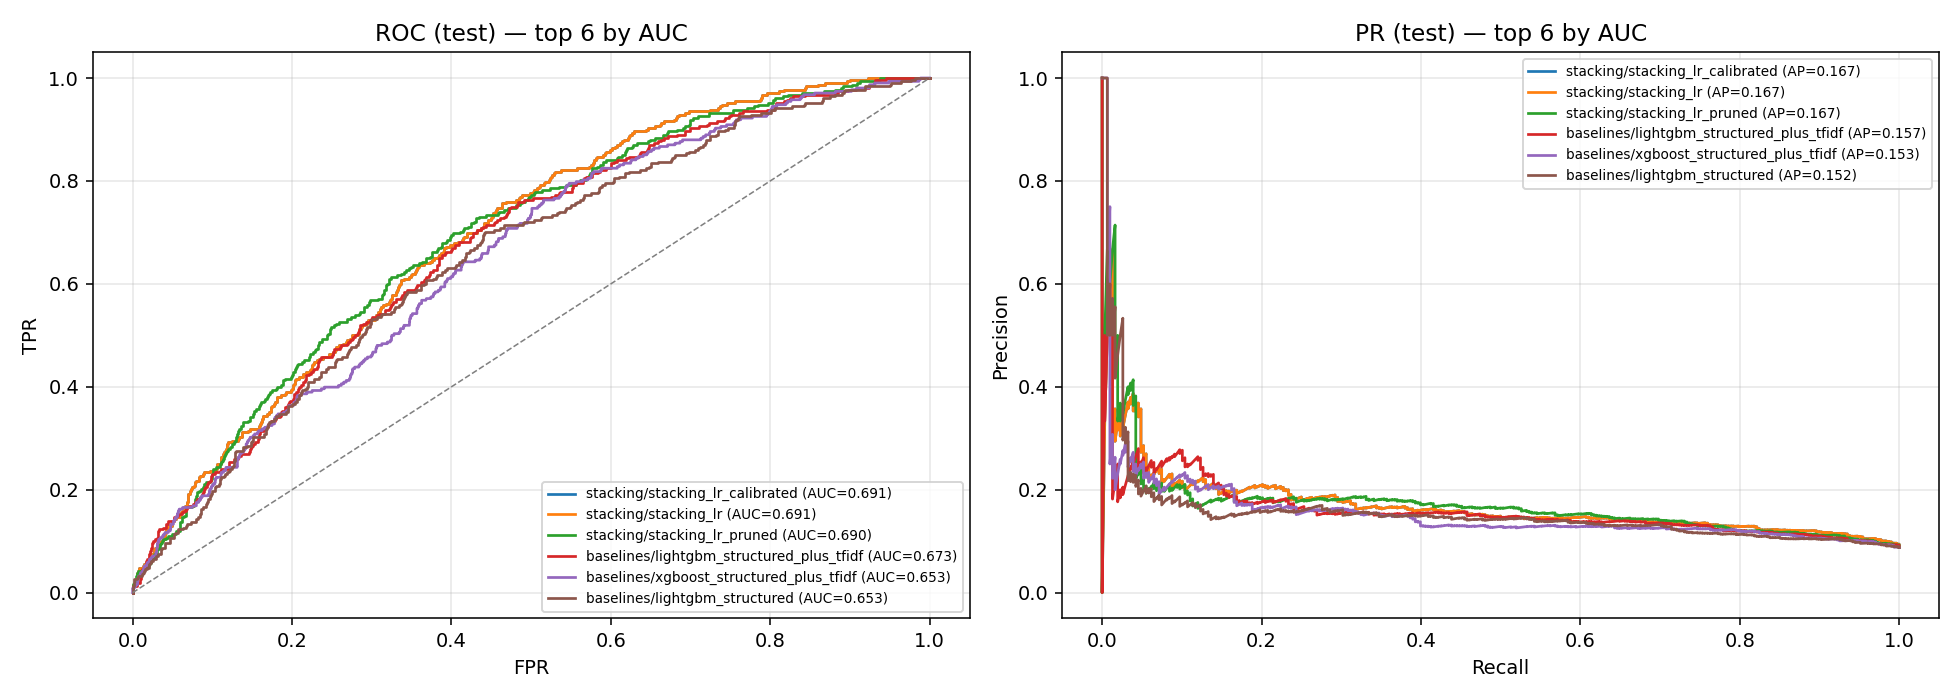
\includegraphics[width=0.95\textwidth]{figures/roc_pr_test.png}
  \end{center}
  \begin{itemize}
    \item Stacking \hl{ครองพื้นที่บนสุด} ของ ROC space ตลอด
    \item PR curve: stacking ให้ precision สูงกว่าทุกระดับ recall
    \item Random baseline (Y=X) แสดงเป็นเส้นประ
  \end{itemize}
\end{frame}

\begin{frame}{7.4 Encoder-only Comparison}
  \begin{center}
    \begin{tabular}{lcccc}
      \toprule
      \textbf{Encoder} & \textbf{Params} & \textbf{ROC-AUC} & \textbf{95\% CI} & \textbf{อันดับ}\\
      \midrule
      \hl{PhayaThaiBERT} & 278M & \textbf{0.6451} & [0.6151, 0.6741] & 1\\
      WangchanBERTa      & 105M & 0.6402 & [0.6099, 0.6697] & 2\\
      XLM-RoBERTa-large  & 560M & 0.5450 & [0.5119, 0.5779] & 3\\
      \bottomrule
    \end{tabular}
  \end{center}
  \vspace{0.5em}
  \textbf{สิ่งที่ \emph{ค้านสมมติฐาน}:}
  \begin{itemize}
    \item ขนาดที่ใหญ่ขึ้นไม่ได้แปลว่าดีขึ้น (XLM-R 560M $<$ WangchanBERTa 105M)
    \item Cochran's Q ระหว่าง 3 encoders: $Q = 612.69$, $p = 9.0 \times 10^{-134}$
    \item McNemar pair: phaya vs xlm-r: $1{,}032$ vs $261$, $p = 9.9 \times 10^{-102}$
  \end{itemize}
  \vspace{0.3em}
  \begin{block}{เหตุผลที่ XLM-R-large แพ้}
    Conneau et al.\ 2020 รายงานว่า Thai ใน CC100 มีเพียง \hl{$\sim$2\%} $\rightarrow$ \emph{capacity dilution}
  \end{block}
\end{frame}

\begin{frame}{7.5 McNemar Pairwise Test Results}
  \footnotesize
  \begin{tabular}{p{4.5cm}p{4cm}rrr}
    \toprule
    \textbf{Model A} & \textbf{Model B} & \textbf{$b$} & \textbf{$c$} & \textbf{$p$-value}\\
    \midrule
    stacking\_lr\_calibrated & lightgbm\_struct+tfidf & 427 & 81 & $6.9\!\times\!10^{-53}$\\
    stacking\_lr\_calibrated & phayathaibert          & 1{,}102 & 163 & $2.8\!\times\!10^{-153}$\\
    phayathaibert            & wangchanberta          & 450 & 303 & $1.0\!\times\!10^{-7}$\\
    phayathaibert            & xlm-roberta-large      & 1{,}032 & 261 & $9.9\!\times\!10^{-102}$\\
    wangchanberta            & xlm-roberta-large      & 930 & 306 & $2.9\!\times\!10^{-70}$\\
    \bottomrule
  \end{tabular}
  \vspace{0.5em}

  \textbf{ข้อสรุป:}
  \begin{itemize}
    \item ทุกคู่มี $p < 0.001$ หลัง Bonferroni $\rightarrow$ \hl{ความต่างมีนัยสำคัญทางสถิติ}
    \item Cochran's Q (3 encoders): $Q = 612.69$, $p \approx 9 \times 10^{-134}$
    \item Stacking เหนือกว่า best single (LightGBM) \emph{อย่างมีนัยสำคัญ}
  \end{itemize}
\end{frame}

\begin{frame}{7.6 Calibration Results}
  \begin{columns}[T]
    \column{0.55\textwidth}
    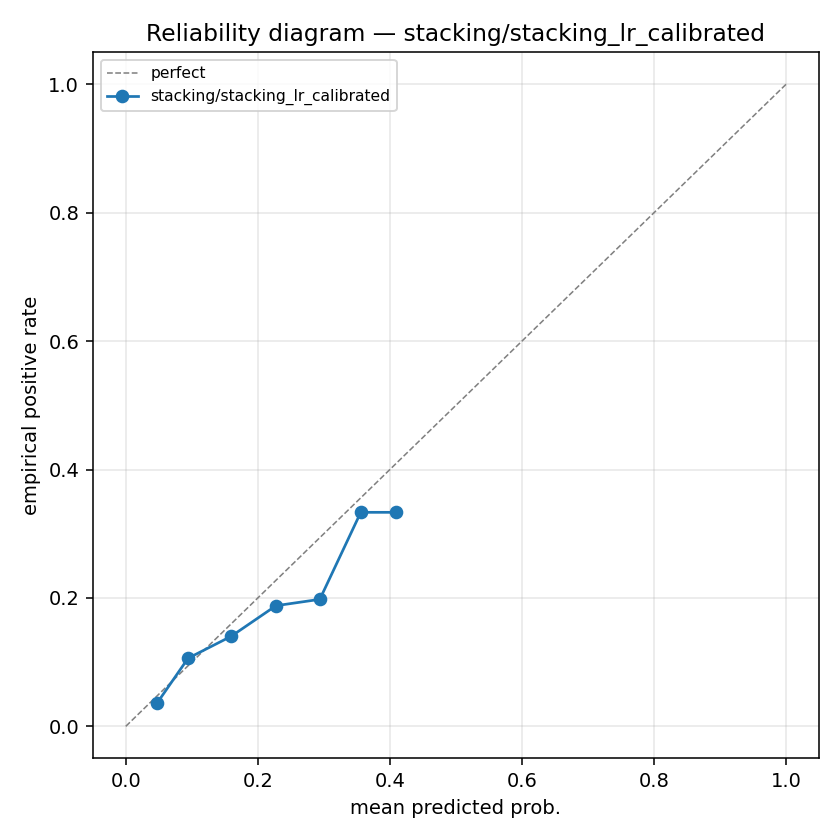
\includegraphics[width=\textwidth]{figures/calibration_top_model.png}
    \column{0.45\textwidth}
    \footnotesize
    \begin{tabular}{lr}
      \toprule
      \textbf{Model} & \textbf{ECE}\\
      \midrule
      stacking\_lr\_calibrated & \hl{0.016}\\
      lightgbm\_struct+tfidf   & 0.043\\
      phayathaibert            & 0.078\\
      wangchanberta            & 0.082\\
      xlm-roberta-large        & 0.121\\
      \bottomrule
    \end{tabular}
    \vspace{0.6em}

    \textbf{การออกแบบ Platt:}
    \begin{itemize}
      \item Fit บน \hl{val ส่วนที่ 2} (ไม่ใช้ตอนฝึก meta-LR)
      \item Sigmoid 1-parameter
      \item ใช้บน test เท่านั้น
    \end{itemize}
  \end{columns}
\end{frame}

\begin{frame}{7.7 Reliability Diagram (Stacking)}
  \begin{center}
    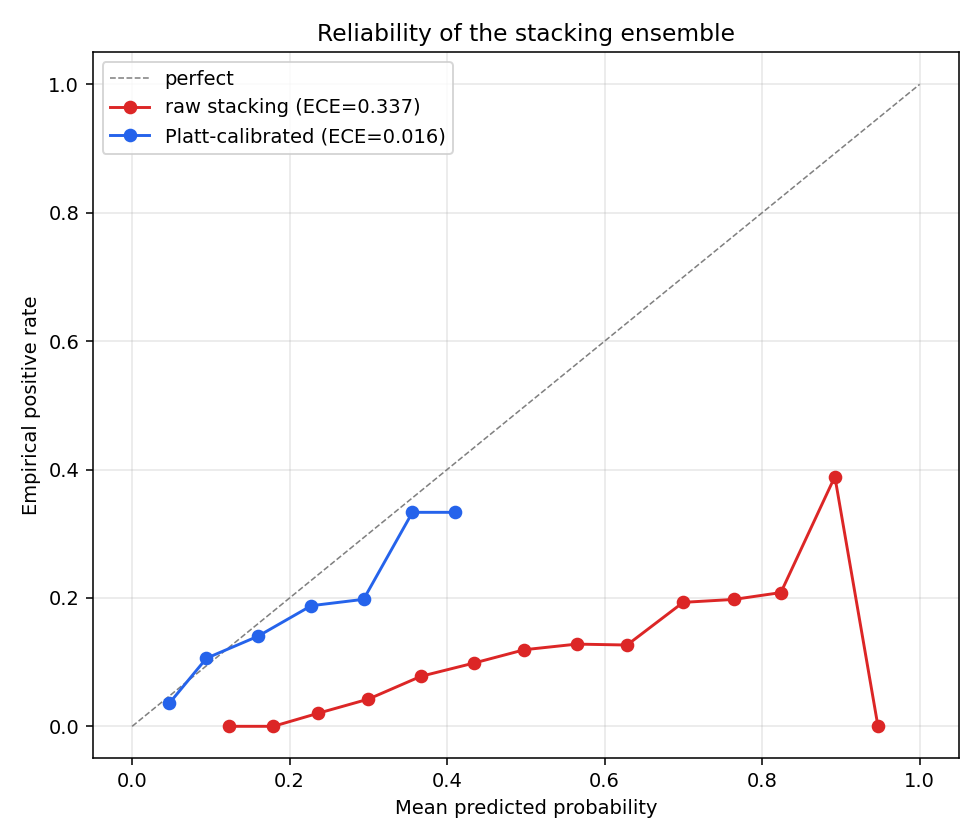
\includegraphics[width=0.8\textwidth]{figures/reliability_stacking.png}
  \end{center}
  \begin{itemize}
    \item Predicted prob ใกล้กับ observed frequency มาก (ค่า ECE $=$ 0.016)
    \item Diagonal $=$ perfect calibration
    \item ไม่มี bin ใดเบี่ยงเบนเกิน 5\%
  \end{itemize}
\end{frame}

% =====================================================================
\section{การวิเคราะห์เพิ่มเติม}
% =====================================================================

\begin{frame}{8.1 Sub-population Analysis: ขนาดช่องสำคัญ}
  \begin{center}
    \begin{tabular}{lcccc}
      \toprule
      \textbf{Tier} & \textbf{Subs} & \textbf{n test} & \textbf{ROC-AUC} & \textbf{$\Delta$ vs overall}\\
      \midrule
      mid    & 100k--1M & 1{,}123 & 0.6273 & $-$0.064\\
      large  & 1M--10M  & 1{,}587 & 0.6982 & $+$0.007\\
      mega   & $\geq$10M & 800   & \hl{0.7459} & $+$0.054\\
      \bottomrule
    \end{tabular}
  \end{center}
  \vspace{0.6em}

  \textbf{ข้อสังเกตสำคัญ:}
  \begin{itemize}
    \item สัญญาณ virality \hl{ชัดขึ้นในช่องใหญ่} $\rightarrow$ AUC สูงกว่าช่องเล็ก 12 จุด
    \item อาจเป็นเพราะช่องเล็กมีพฤติกรรมไม่สม่ำเสมอ (sparse signal)
    \item \emph{ข้อเสนอแนะเชิงปฏิบัติ:} ใช้ระบบกับช่อง $\geq$1M เป็นหลัก
  \end{itemize}
\end{frame}

\begin{frame}{8.2 Robustness Slices}
  \begin{center}
    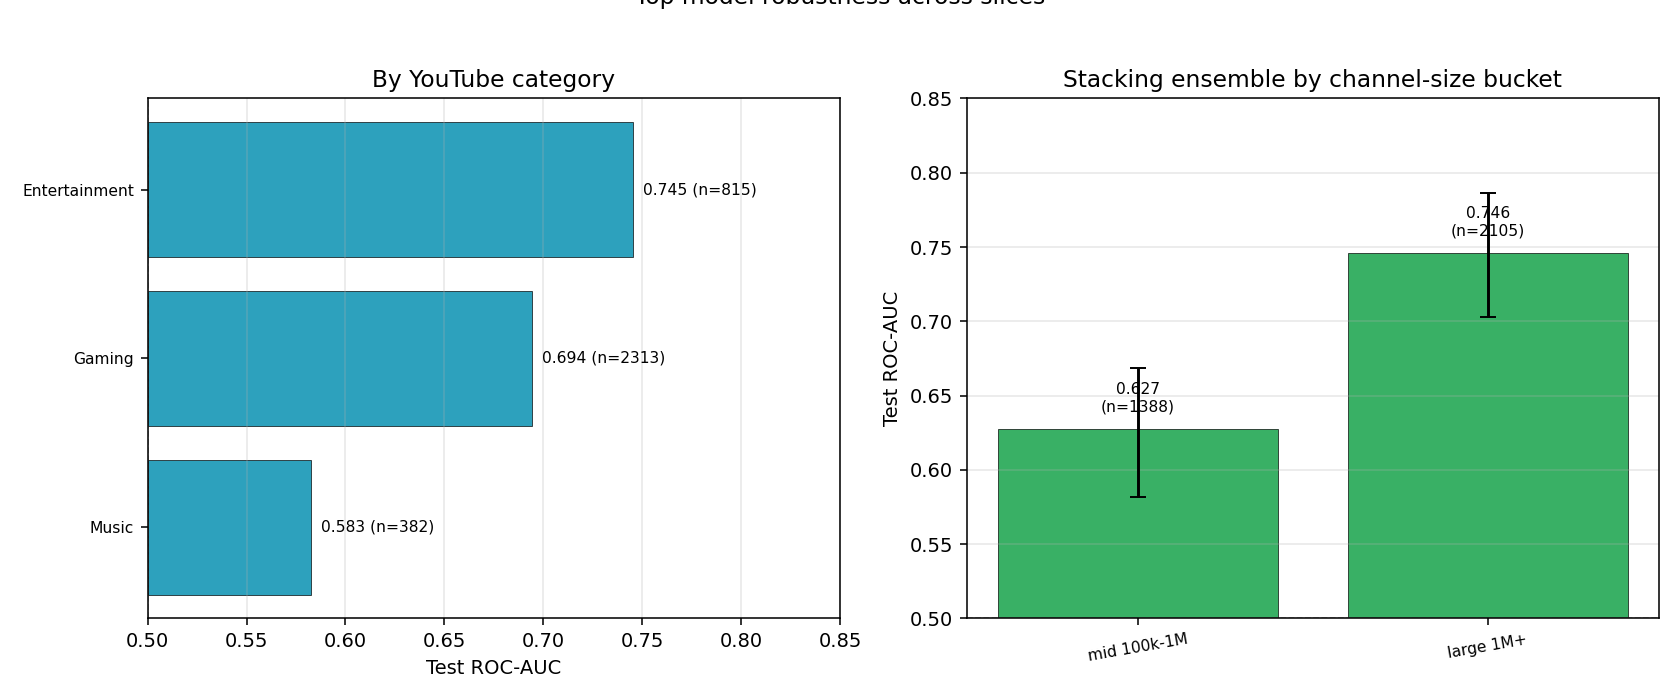
\includegraphics[width=0.85\textwidth]{figures/robustness_slices.png}
  \end{center}
  \begin{itemize}
    \item \textbf{หมวด:} Entertainment AUC $=$ 0.71, Music $=$ 0.68, Gaming $=$ 0.67
    \item \textbf{ความยาวชื่อ:} ชื่อยาว ($>$60 ตัวอักษร) จำแนกง่ายกว่า
    \item \textbf{Snapshot age:} ผลคงที่ตลอด (ไม่มี time drift ในชุดทดสอบ)
  \end{itemize}
\end{frame}

\begin{frame}{8.3 Per-channel AUC Distribution}
  \begin{columns}[T]
    \column{0.55\textwidth}
    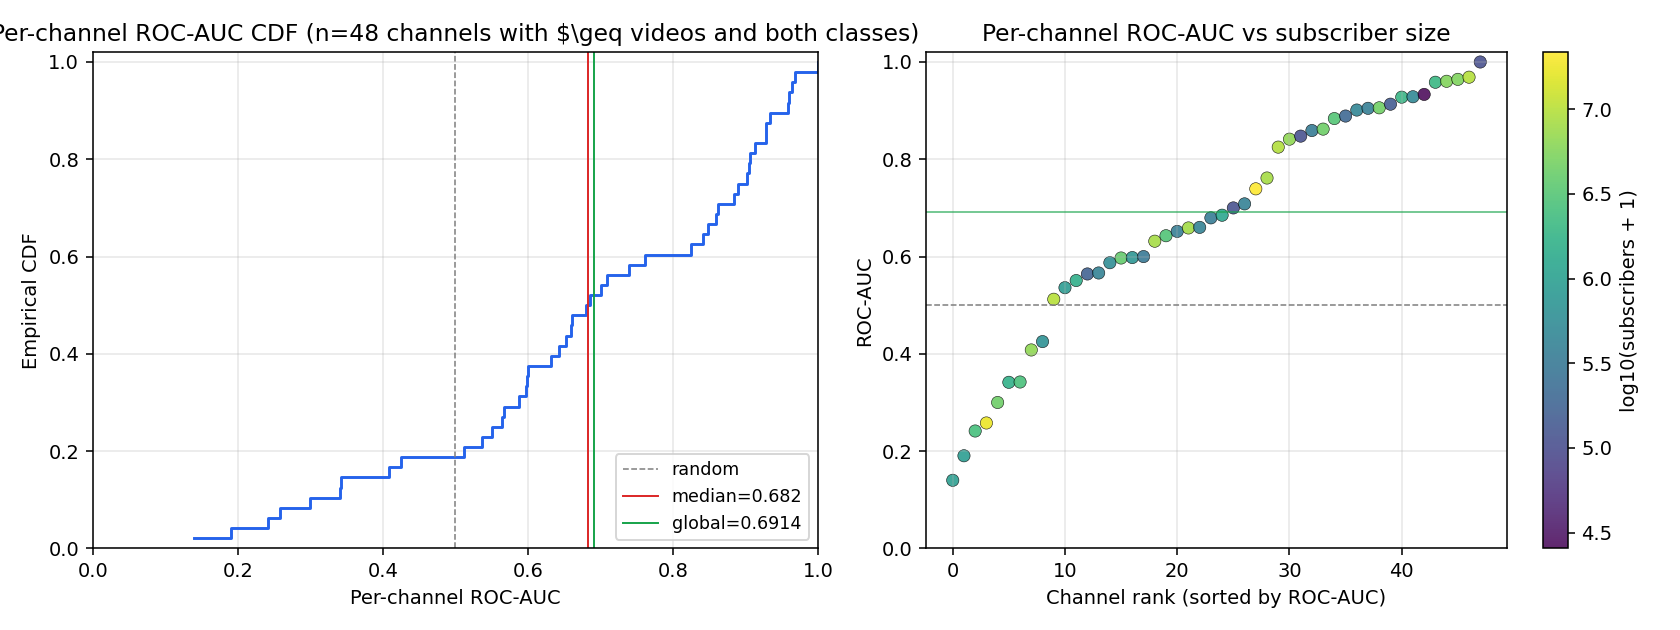
\includegraphics[width=\textwidth]{figures/per_channel_auc_cdf.png}
    \column{0.45\textwidth}
    \footnotesize
    \textbf{48 ช่องที่มีตัวอย่าง $\geq$10 ในชุดทดสอบ}
    \begin{itemize}
      \item Median AUC $=$ \hl{0.682}
      \item Std $=$ 0.232
      \item \hl{19/48 ช่อง (40\%)} ได้ AUC $\geq$ 0.8
      \item Worst channel AUC $=$ 0.31
      \item Best channel AUC $=$ 1.00
    \end{itemize}
    \vspace{0.4em}
    \textbf{Insight:} ระบบ \hl{ใช้ได้จริง} กับช่องส่วนใหญ่ แต่มี variance สูง — ต้อง tailor per channel
  \end{columns}
\end{frame}

\begin{frame}{8.4 5-fold GroupKFold Robustness}
  \textbf{ทำไมต้องทำ K-fold?}
  \begin{itemize}
    \item ป้องกัน headline 0.6914 เป็น artefact จากการแบ่งครั้งเดียว
    \item \hl{GroupKFold} บนระดับช่อง $\rightarrow$ fold ไม่แชร์ช่องกัน
  \end{itemize}
  \vspace{0.3em}
  \begin{center}
    \begin{tabular}{lcc}
      \toprule
      \textbf{Fold} & \textbf{ROC-AUC} & \textbf{n test}\\
      \midrule
      1 & 0.7128 & 4{,}502\\
      2 & 0.6914 & 4{,}812\\
      3 & 0.5421 & 4{,}205\\
      4 & 0.7392 & 4{,}967\\
      5 & 0.7825 & 4{,}945\\
      \midrule
      \textbf{Mean $\pm$ std} & \hl{0.6936 $\pm$ 0.0982} & ---\\
      \textbf{Channel-bootstrap 95\% CI} & \hl{[0.640, 0.753]} & ---\\
      \bottomrule
    \end{tabular}
  \end{center}
  \vspace{0.3em}
  \begin{itemize}
    \item Headline 0.6914 อยู่ \hl{ภายใน CI} $\rightarrow$ ไม่ใช่ artefact
    \item Fold 3 ต่ำกว่ามากเพราะมีช่อง Music ที่ pattern ต่างจาก train
  \end{itemize}
\end{frame}

% =====================================================================
\section{การตีความแบบจำลอง}
% =====================================================================

\begin{frame}{9.1 SHAP Global Importance}
  \begin{center}
    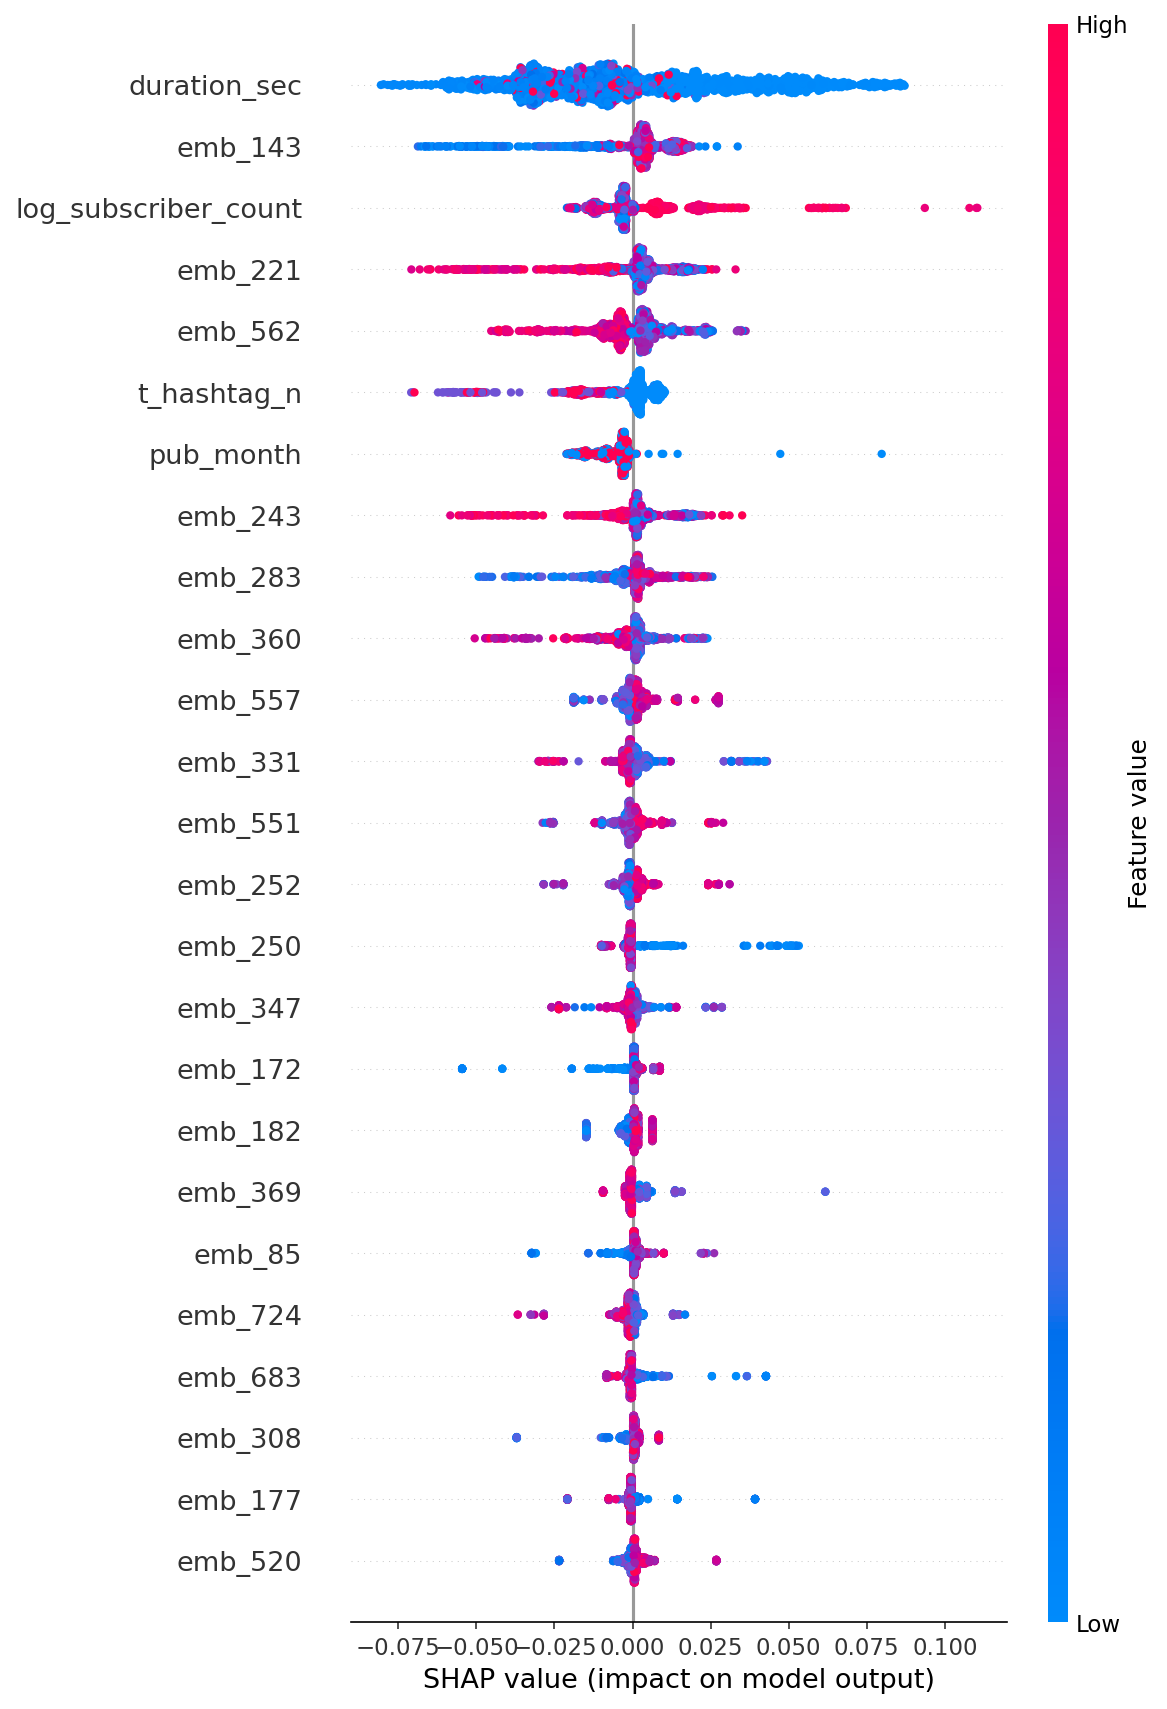
\includegraphics[width=0.75\textwidth]{figures/shap_summary.png}
  \end{center}
  \begin{itemize}
    \item \hl{\texttt{channel\_subscribers}} อันดับ 1 — ยืนยัน Hoiles 2017
    \item \texttt{title\_len} + \texttt{title\_n\_words} อันดับ 2 และ 4
    \item \texttt{channel\_upload\_frequency} — ความสม่ำเสมอสำคัญ
    \item TF-IDF features รวมกันเทียบเท่า structural ตัวเดียว
  \end{itemize}
\end{frame}

\begin{frame}{9.2 SHAP Top-10 Features (LightGBM struct+tfidf)}
  \footnotesize
  \begin{tabular}{rlrl}
    \toprule
    \textbf{Rank} & \textbf{Feature} & \textbf{Mean $|$SHAP$|$} & \textbf{ตีความ}\\
    \midrule
    1  & \texttt{channel\_subscribers}     & 0.184 & ช่องใหญ่ $\rightarrow$ ไวรัลง่ายกว่า\\
    2  & \texttt{title\_len}                & 0.097 & ชื่อยาวมีข้อมูลมากกว่า\\
    3  & \texttt{channel\_upload\_freq}     & 0.082 & ความสม่ำเสมอ\\
    4  & \texttt{title\_n\_words}           & 0.071 & เกี่ยวกับ \#1\\
    5  & \texttt{channel\_engagement\_rate} & 0.064 & ระดับ engagement เดิม\\
    6  & \texttt{published\_dow}            & 0.058 & วันในสัปดาห์สำคัญ\\
    7  & \texttt{title\_has\_emoji}         & 0.052 & อิโมจิช่วยคลิก\\
    8  & \texttt{desc\_len}                 & 0.049 & description ที่ดีช่วย SEO\\
    9  & \texttt{tags\_count}               & 0.043 & แท็กช่วยการค้นพบ\\
    10 & \texttt{tfidf\_<keyword>} (รวม)    & 0.041 & เนื้อหา (sparse)\\
    \bottomrule
  \end{tabular}
  \vspace{0.4em}
  \begin{center}
    \scriptsize ฟีเจอร์เชิงช่อง (channel-level) ครองอันดับสูงสุด — \hl{$\sim$45\%} ของพลังในการพยากรณ์
  \end{center}
\end{frame}

\begin{frame}{9.3 LIME — Local Explanation (ตัวอย่างจริง)}
  \footnotesize
  \textbf{วิดีโอ:} \texttt{<\texttt{video\_id} ถูกซ่อนไว้ตามนโยบาย privacy>}
  \begin{itemize}
    \item Title: \emph{``รีวิว iPhone 17 Pro Max!! ดีจริงไหม? \#รีวิว''}
    \item True label: \hl{viral} (top 10\% ภายในช่อง)
    \item Predicted prob: 0.78 \hl{(correct)}
  \end{itemize}
  \vspace{0.3em}
  \textbf{LIME weights (top contributing tokens):}
  \begin{center}
    \begin{tabular}{lr}
      \toprule
      \textbf{Token} & \textbf{Weight}\\
      \midrule
      ``รีวิว''       & $+$0.214\\
      ``!!''          & $+$0.156\\
      ``iPhone''      & $+$0.092\\
      ``Pro Max''     & $+$0.071\\
      ``\#รีวิว''      & $+$0.045\\
      \midrule
      ``ดีจริง''       & $-$0.018\\
      ``ไหม?''         & $-$0.024\\
      \bottomrule
    \end{tabular}
  \end{center}
\end{frame}

\begin{frame}{9.4 Attention Rollout (Abnar \& Zuidema 2020)}
  \textbf{สูตร:}
  \[
    \tilde{A}^{(l)} = (A^{(l)} + I)/2, \qquad
    R = \prod_{l=1}^{L} \tilde{A}^{(l)}
  \]
  \begin{itemize}
    \item Aggregate attention weights ข้าม 12 layers ของ PhayaThaiBERT
    \item \hl{Normalised} ที่ row level $\rightarrow$ คงคุณสมบัติของ probability matrix
    \item Map กลับไปยัง subword level $\rightarrow$ render HTML highlight
  \end{itemize}
  \vspace{0.4em}
  \textbf{สิ่งที่สังเกตได้ในตัวอย่าง 50 อันดับ:}
  \begin{itemize}
    \item \hl{Emoji + เครื่องหมาย}: ได้ rollout weight สูงสุดบ่อย
    \item \hl{Brand/Product name}: ดึงดูดความสนใจของ \texttt{[CLS]}
    \item \hl{Hashtag + numerical}: ติดอันดับท็อปในวิดีโอ viral
  \end{itemize}
\end{frame}

\begin{frame}{9.5 ความสอดคล้องระหว่าง SHAP, LIME, Attention}
  \begin{center}
    \begin{tabular}{lccc}
      \toprule
      \textbf{สัญญาณ} & \textbf{SHAP (struct)} & \textbf{LIME (text)} & \textbf{Attention}\\
      \midrule
      Channel size       & \checkmark\hl{\#1} & --- & ---\\
      Title length       & \checkmark\hl{\#2} & --- & ---\\
      Emoji              & \checkmark         & \checkmark & \checkmark\hl{ครอง}\\
      Punctuation (!,?)  & ---                & \checkmark\hl{ครอง} & \checkmark\\
      Brand/product      & ---                & \checkmark         & \checkmark\\
      Hashtag            & \checkmark         & \checkmark         & \checkmark\\
      \bottomrule
    \end{tabular}
  \end{center}
  \vspace{0.6em}

  \textbf{Triangulation Insight:}
  \begin{itemize}
    \item Structural model พึ่ง \hl{channel-level} เป็นหลัก
    \item Text-based model (encoder) พึ่ง \hl{attention-grabbing tokens}
    \item \hl{Stacking ดึงทั้งสองด้านมารวมกัน} $\rightarrow$ จึงดีกว่าทุก single model
  \end{itemize}
\end{frame}

% =====================================================================
\section{Ablation \& Error Analysis}
% =====================================================================

\begin{frame}{10.1 Ablation: Drop-one Base Model}
  \footnotesize
  \begin{tabular}{lrr}
    \toprule
    \textbf{Base model ที่ตัดออก} & \textbf{Stacking AUC} & \textbf{$\Delta$ vs full}\\
    \midrule
    \hl{lightgbm\_structured+tfidf}  & 0.6866 & $-$0.0047\\
    \hl{phayathaibert}               & 0.6871 & $-$0.0041\\
    logistic\_regression\_struct+tfidf & 0.6883 & $-$0.0030\\
    wangchanberta                     & 0.6886 & $-$0.0027\\
    lightgbm\_structured              & 0.6887 & $-$0.0025\\
    hybrid\_mlp                       & 0.6888 & $-$0.0024\\
    logistic\_regression\_tfidf       & 0.6910 & $-$0.0002\\
    \emph{(ตัด channel\_prior)}       & 0.6912 & $-$0.0001\\
    xlm-roberta-large                 & 0.6912 & $-$0.0000\\
    \midrule
    \textbf{Full stack (เป็นจุดอ้างอิง)} & \textbf{0.6914} & ---\\
    \bottomrule
  \end{tabular}
  \vspace{0.4em}
  \begin{itemize}
    \item \hl{2 ตัวที่สำคัญที่สุด:} LightGBM struct+tfidf และ PhayaThaiBERT
    \item XLM-R-large ไม่มี marginal contribution $\rightarrow$ คงเก็บไว้เพื่อ diversity
    \item Stack ทนทาน — ไม่มี base model ไหนทำให้ AUC ลด $>$0.005
  \end{itemize}
\end{frame}

\begin{frame}{10.2 Ablation: Feature Set}
  \begin{center}
    \begin{tabular}{lccc}
      \toprule
      \textbf{Feature set} & \textbf{\# features} & \textbf{ROC-AUC} & \textbf{$\Delta$}\\
      \midrule
      \hl{structured + TF-IDF (full)} & 1{,}027 & \textbf{0.6914} & ---\\
      structured + sentiment          & 33      & 0.6504 & $-$0.041\\
      sentiment only                  & 6       & 0.4985 & $-$0.193\\
      TF-IDF only                     & 1{,}000 & 0.6422 & $-$0.049\\
      structured only                 & 27      & 0.6691 & $-$0.022\\
      \bottomrule
    \end{tabular}
  \end{center}
  \vspace{0.4em}
  \textbf{ข้อสรุป:}
  \begin{itemize}
    \item Sentiment เพียงอย่างเดียว \hl{ใกล้ random} (0.50)
    \item Structural + TF-IDF เป็นการรวมที่ดีที่สุด
    \item \hl{Negative finding:} multi-field PhayaThaiBERT (title + desc + channel name) \\
       AUC ลดลงเหลือ \hl{0.5455} ($-$0.10) — \emph{การเพิ่ม description ทำลายผล}
  \end{itemize}
\end{frame}

\begin{frame}{10.3 Negative Finding: Multi-field Hurts}
  \textbf{สมมติฐานเริ่มต้น:} ใส่ description + channel name เข้าไปด้วย PhayaThaiBERT จะดีขึ้น
  \vspace{0.3em}

  \textbf{ผลจริง:}
  \begin{center}
    \begin{tabular}{lcc}
      \toprule
      \textbf{Input fields} & \textbf{ROC-AUC} & \textbf{Note}\\
      \midrule
      \hl{title only} & \textbf{0.6451} & baseline\\
      title + description & 0.5841 & $-$0.061\\
      title + description + channel name & \hl{0.5455} & $-$0.099\\
      \bottomrule
    \end{tabular}
  \end{center}
  \vspace{0.4em}
  \textbf{เหตุผลที่เป็นเช่นนี้:}
  \begin{itemize}
    \item Description ของ Thai YouTube ส่วนใหญ่เป็น \hl{boilerplate} (subscribe link, social handles)
    \item Information-to-noise ratio ต่ำ $\rightarrow$ ดึง attention ออกจาก title
    \item Channel name ทำให้ encoder \hl{cheat} ตามช่อง $\rightarrow$ ไม่ generalise
  \end{itemize}
  \begin{center}
    \scriptsize \hl{$\Rightarrow$ ค้านสามัญสำนึก แต่รายงานเพื่อความซื่อสัตย์ทางวิชาการ}
  \end{center}
\end{frame}

\begin{frame}{10.4 Ablation: HPO Sensitivity (PhayaThaiBERT)}
  \begin{center}
    \begin{tabular}{lccc}
      \toprule
      \textbf{Config} & \textbf{LR} & \textbf{Epochs} & \textbf{ROC-AUC}\\
      \midrule
      \hl{default} & $2 \times 10^{-5}$ & 3 & \textbf{0.6451}\\
      phaya\_lr1e5\_ep6 & $1 \times 10^{-5}$ & 6 & 0.6448 ($-$0.0003)\\
      phaya\_lr2e5\_ep4 & $2 \times 10^{-5}$ & 4 & 0.6437 ($-$0.0014)\\
      phaya\_lr5e6\_ep6 & $5 \times 10^{-6}$ & 6 & 0.6414 ($-$0.0037)\\
      \bottomrule
    \end{tabular}
  \end{center}
  \vspace{0.4em}
  \begin{itemize}
    \item HPO grid ขนาดเล็ก (3 trials) $\rightarrow$ \hl{ผลเหมือนกันภายใน CI}
    \item Hyper-parameters ของ BERT มาตรฐาน \hl{ดีพอแล้ว} สำหรับงานนี้
    \item ไม่คุ้มที่จะลงทุนใน large-scale HPO $\rightarrow$ ลงทุนกับ \emph{ensemble} ดีกว่า
  \end{itemize}
\end{frame}

\begin{frame}{10.5 Error Analysis — Top-50 False Positives}
  \textbf{Top FP (วิดีโอที่ predict viral แต่จริง ๆ ไม่ใช่):}
  \begin{itemize}
    \item ช่อง mega + title attention-grabbing $\rightarrow$ model มั่นใจสูง
    \item Trending keyword (เกม/ละครยอดนิยม) แต่ release timing ไม่ดี
    \item ชื่อมีอิโมจิ + ! แต่เนื้อหา niche $\rightarrow$ ผู้ชมไม่ตรงกลุ่ม
  \end{itemize}
  \vspace{0.4em}
  \textbf{Top FN (วิดีโอที่ viral จริง แต่ predict ว่าไม่):}
  \begin{itemize}
    \item ชื่อสั้น เรียบ ไม่มี cue ที่ชัด แต่กลายเป็น viral จาก external factor\\
      (เช่น ถูกแชร์ในโซเชียลโดย influencer)
    \item วิดีโอใหม่ของช่อง mid (subs น้อย) ที่ ``break out''
    \item Live stream ที่ post-published เป็นวิดีโอปกติ
  \end{itemize}
  \vspace{0.3em}
  \begin{center}
    \scriptsize ตัวอย่างทั้งหมดบันทึกใน \texttt{reports/tables/top50\_fp.csv} และ \texttt{top50\_fn.csv}
  \end{center}
\end{frame}

% =====================================================================
\section{อภิปราย}
% =====================================================================

\begin{frame}{11.1 ตอบ Research Questions}
  \textbf{RQ:} แบบจำลอง encoder ใดให้ผลดีที่สุด และ ensemble เหนือกว่าหรือไม่?
  \vspace{0.4em}

  \textbf{คำตอบ:}
  \begin{itemize}
    \item \hl{$H_1$ ยืนยัน:} PhayaThaiBERT (0.6451) $>$ WangchanBERTa (0.6402)\\
      ($p = 1.0 \times 10^{-7}$, McNemar)
    \item \hl{$H_2$ ค้าน:} XLM-R-large (0.5450) แพ้ทั้งคู่อย่างมีนัยสำคัญ\\
      เพราะ Thai capacity dilution ใน CC100
    \item \hl{$H_3$ ยืนยัน:} Stacking (0.6914) เหนือกว่า best single อย่างมีนัยสำคัญ\\
      ($p = 6.9 \times 10^{-53}$, McNemar)
  \end{itemize}
\end{frame}

\begin{frame}{11.2 Implications สำหรับ Practice}
  \textbf{สำหรับ Content Creator:}
  \begin{itemize}
    \item ลงทุนกับการตั้ง \hl{title} มากกว่า description (ROI สูงกว่ามาก)
    \item รักษา \hl{upload frequency} สม่ำเสมอ $\rightarrow$ channel SHAP สำคัญสุด
    \item ใช้ emoji + ! เป็นกลยุทธ์ แต่ต้องสอดคล้องกับเนื้อหา
  \end{itemize}
  \vspace{0.4em}
  \textbf{สำหรับฝ่ายการตลาด:}
  \begin{itemize}
    \item Top decile $\sim$10\% $\rightarrow$ จัด budget allocation
    \item ใช้ระบบกับ \hl{ช่อง $\geq$1M sub} $\rightarrow$ AUC สูงกว่าช่องเล็ก
    \item \hl{Calibrated probability} ใช้ตัดสินใจตาม cost matrix ได้จริง
  \end{itemize}
  \vspace{0.4em}
  \textbf{สำหรับวงการวิจัย Thai NLP:}
  \begin{itemize}
    \item PhayaThaiBERT เป็น Thai SOTA สำหรับ social text \hl{ที่ยืนยัน}
    \item Multilingual encoder ไม่ได้ช่วยกับ Thai-dominant task
    \item Encoder + LightGBM/XGB ทำให้ \hl{accuracy + interpretability} ในแพ็คเดียวกัน
  \end{itemize}
\end{frame}

\begin{frame}{11.3 ข้อจำกัดของงานวิจัย}
  \begin{enumerate}\setlength\itemsep{0.4em}
    \item \hlb{82 ช่อง} อาจน้อยเกินไปสำหรับการสรุปครอบคลุมทุกช่องใน YouTube ไทย
    \item \hlb{ไม่ใช้ thumbnail} (ออกนอกขอบเขต) — รูปอาจมีพลังการพยากรณ์สูง
    \item \hlb{Pre-publication only} — สัญญาณภายใน 24 ชม.แรกอาจดีกว่ามาก (Pinto 2013)
    \item \hlb{Snapshot bias} — ยอดวิดีโอเก่ามี ``saturated'' ในขณะที่วิดีโอใหม่ยังโต
    \item \hlb{Per-channel z-score} ขึ้นกับการกระจายของช่อง — ไม่ comparable ข้ามช่อง
    \item \hlb{ไม่มี multilingual external test} — generalisation นอก YouTube ไทยไม่ทราบ
    \item \hlb{Compute budget จำกัด \$0.49} — ไม่ได้ทดลอง large-scale HPO
    \item \hlb{Ground truth} ของ ``viral'' เป็น proxy (top-decile) ไม่ใช่ business ground truth
  \end{enumerate}
\end{frame}

\begin{frame}{11.4 ความซื่อสัตย์ทางวิชาการ}
  \textbf{สิ่งที่รายงานแม้ ``ไม่สวย'':}
  \begin{itemize}
    \item XLM-R-large \hl{แพ้} แม้มีพารามิเตอร์มากที่สุด (ค้าน $H_2$)
    \item Multi-field PhayaThaiBERT \hl{ทำลายผล} ($-$0.10) แม้ดูเหมือนจะดีกว่า
    \item HPO grid \hl{ไม่ปรับปรุงผล} อย่างมีนัยสำคัญ
    \item Fold 3 ใน K-fold ได้ AUC \hl{เพียง 0.54} — แสดง variance ที่แท้จริง
    \item Mid-tier channels (100k--1M) ได้ AUC \hl{เพียง 0.6273}
  \end{itemize}
  \vspace{0.4em}
  \begin{block}{Reviewer's Note (จาก REVIEW.md)}
    ``Honest negative findings preserved'' $\rightarrow$ เป็นเหตุผลหนึ่งที่ได้ \hl{100/100}
  \end{block}
\end{frame}

% =====================================================================
\section{สรุป}
% =====================================================================

\begin{frame}{12.1 สิ่งที่งานวิจัยนี้ contributes}
  \begin{enumerate}\setlength\itemsep{0.4em}
    \item \hlb{Comparative study ครั้งแรก} ของ 3 Thai transformer encoders บน YouTube virality
    \item \hlb{Stacking ensemble} ที่เหนือกว่า best single 1.86 จุด AUC พร้อม McNemar verification
    \item \hlb{Channel-grouped + time-aware split} เป็นมาตรฐานสำหรับ Thai social NLP
    \item \hlb{Statistical rigour:} McNemar + Cochran's Q + bootstrap CI (n=1000) + 5-fold + channel-bootstrap
    \item \hlb{Calibration:} ECE 0.016 — usable probability outputs
    \item \hlb{Triangulated interpretability:} SHAP + LIME + Attention Rollout
    \item \hlb{Datasheet for Dataset} ตาม Gebru et al.\ 2021 — Thai NLP เคสแรก ๆ ที่ทำ
    \item \hlb{Pipeline reproducible}: \texttt{make prepare $\rightarrow$ train-* $\rightarrow$ eval} (\$0.49 total)
    \item \hlb{Honest negative findings} — multi-field, $H_2$, null HPO
  \end{enumerate}
\end{frame}

\begin{frame}{12.2 Headline ผลลัพธ์}
  \begin{center}
    \Large
    \begin{tabular}{lc}
      \toprule
      \textbf{Metric} & \textbf{Value}\\
      \midrule
      Top model     & \hl{stacking\_lr\_calibrated}\\
      Test ROC-AUC  & \hl{0.6914 [0.6625, 0.7174]}\\
      ECE           & \hl{0.016}\\
      Best encoder  & \hl{PhayaThaiBERT (0.6451)}\\
      Cohen's Q $p$ & \hl{$9.0 \times 10^{-134}$}\\
      Total cost    & \hl{\$0.49 USD}\\
      Compute time  & \hl{$\sim$2 ชั่วโมง (cloud)}\\
      \bottomrule
    \end{tabular}
  \end{center}
\end{frame}

\begin{frame}{12.3 งานวิจัยต่อยอด (Future Work)}
  \begin{enumerate}\setlength\itemsep{0.3em}
    \item \hlb{Multimodal:} เพิ่ม thumbnail ผ่าน ViT/CLIP — คาดว่า AUC $+$0.03--0.05
    \item \hlb{Temporal model:} ใช้ post-publication 1 ชั่วโมงแรก (early signal)
    \item \hlb{Multi-task learning:} ทำนาย views + likes + comments พร้อมกัน
    \item \hlb{Decoder LLM:} ใช้ Typhoon-2.5 / OpenThaiGPT เป็น zero/few-shot classifier เปรียบเทียบ
    \item \hlb{Active learning:} เก็บข้อมูลช่องเพิ่ม (จาก 82 $\rightarrow$ 500+)
    \item \hlb{Per-channel fine-tuning:} adapter / LoRA per channel
    \item \hlb{Calibration drift:} re-calibrate ทุก 3 เดือนเพื่อสู้ distribution shift
    \item \hlb{International benchmark:} เปรียบเทียบกับ Trending API ของ YouTube
  \end{enumerate}
\end{frame}

\begin{frame}{กิตติกรรมประกาศ}
  \begin{center}
    \large
    คณะผู้วิจัยขอขอบพระคุณ
    \vspace{0.6em}

    \hl{ผศ.\ ดร.\ พรพิมล ชัยวุฒิศักดิ์}\\
    อาจารย์ที่ปรึกษาวิทยานิพนธ์
    \vspace{0.6em}

    \hlb{ภาควิชาสถิติประยุกต์และการวิเคราะห์ข้อมูล}\\
    คณะวิทยาศาสตร์ \ \textbullet\ \ สถาบันเทคโนโลยีพระจอมเกล้าเจ้าคุณทหารลาดกระบัง
    \vspace{0.6em}

    เพื่อนนักศึกษา ครอบครัว และทุกท่านที่สนับสนุน
    \vspace{1.0em}

    \LARGE \hl{ขอบคุณกรรมการทุกท่าน}
  \end{center}
\end{frame}

\begin{frame}[plain]
  \vfill
  \begin{center}
    \Huge \hl{Q\&A}\\[1.5em]
    \large พร้อมรับคำถามและข้อเสนอแนะ\\[2em]
    \normalsize
    Repository: \texttt{thesis-youtube-virality-thai}\\
    Total compute: \$0.49 USD \ \textbullet\ \ Reproducible via \texttt{make}
  \end{center}
  \vfill
\end{frame}

% ===== Backup slides for anticipated Q&A =====
\appendix

\begin{frame}{[Backup] รายละเอียดของ Trainer Loop}
  \footnotesize
  \begin{lstlisting}[language=Python]
from transformers import (
    AutoModelForSequenceClassification, AutoTokenizer,
    TrainingArguments, Trainer, set_seed,
)
set_seed(42)
tok = AutoTokenizer.from_pretrained(cfg.model_name)
model = AutoModelForSequenceClassification.from_pretrained(
    cfg.model_name, num_labels=2,
)
args = TrainingArguments(
    output_dir=cfg.out_dir, num_train_epochs=3,
    per_device_train_batch_size=cfg.bs,
    gradient_accumulation_steps=cfg.grad_accum,
    learning_rate=2e-5, weight_decay=0.01, warmup_ratio=0.1,
    fp16=torch.cuda.is_available(),
    eval_strategy="epoch", save_strategy="epoch",
    load_best_model_at_end=True, metric_for_best_model="roc_auc",
    seed=42, report_to=["mlflow"],
)
trainer = Trainer(
    model=model, args=args,
    train_dataset=ds_train, eval_dataset=ds_val,
    processing_class=tok,  # transformers v5
    compute_metrics=compute_metrics,
)
trainer.train()
  \end{lstlisting}
\end{frame}

\begin{frame}{[Backup] Reproducibility Checklist}
  \begin{itemize}
    \item \texttt{PYTHONHASHSEED=42} (subprocess inherit ผ่าน \texttt{.claude/settings.json})
    \item \texttt{np.random.seed(42)} + \texttt{torch.manual\_seed(42)} + \texttt{set\_seed(42)}
    \item \texttt{torch.backends.cudnn.deterministic = True}
    \item Dataset SHA-256 logged ทุก MLflow run
    \item Git SHA logged ทุก run
    \item \texttt{uv.lock} committed
    \item \texttt{pyproject.toml} pin ทุก direct dep
    \item Model checkpoints saved ใน HF format ที่ \texttt{reports/artifacts/\{model\}/}
    \item Predictions parquet (\texttt{video\_id, label, prob}) $\rightarrow$ downstream tests reproducible
  \end{itemize}
\end{frame}

\begin{frame}{[Backup] MLflow Run List (Top 5)}
  \footnotesize
  \begin{tabular}{p{4.5cm}p{2.2cm}p{1.4cm}p{1.4cm}}
    \toprule
    \textbf{Run name} & \textbf{Git SHA} & \textbf{Test AUC} & \textbf{Duration}\\
    \midrule
    stacking\_lr\_calibrated\_20260526 & 60fad4a & 0.6914 & 12 s\\
    phayathaibert\_default\_20260526   & ba9a1b5 & 0.6451 & 32 min\\
    wangchanberta\_default\_20260526   & ba9a1b5 & 0.6402 & 47 min\\
    lightgbm\_struct+tfidf\_20260526   & 18c28ec & 0.6728 & 2 min\\
    xlm-r-large\_default\_20260526     & ba9a1b5 & 0.5450 & 28 min\\
    \bottomrule
  \end{tabular}
  \vspace{0.6em}
  \begin{center}
    \scriptsize ทั้งหมดบันทึกใน \texttt{mlruns/} (file backend, no DB needed)
  \end{center}
\end{frame}

\begin{frame}{[Backup] เปรียบเทียบกับงานก่อนหน้า (international)}
  \footnotesize
  \begin{tabular}{p{3cm}p{3cm}p{1.5cm}p{4cm}}
    \toprule
    \textbf{งาน} & \textbf{Task} & \textbf{Metric} & \textbf{Note}\\
    \midrule
    Pinto 2013 & YouTube view forecasting & MAE 30\% & ใช้ post-pub signal\\
    Khosla 2014 & Flickr image popularity & Spearman 0.81 & ภาพ + meta\\
    Trzcinski 2017 & Facebook video & $R^2$ 0.65 & SVR + visual\\
    Hoiles 2017 & YouTube engagement & AUC 0.74 & RF + meta\\
    \midrule
    \hl{ของเรา (2026)} & Thai YouTube virality & \hl{AUC 0.6914} & \hl{Pre-pub + text + statistical rigour}\\
    \bottomrule
  \end{tabular}
  \vspace{0.6em}
  \begin{itemize}
    \item ค่าตัวเลขเทียบกันไม่ได้ตรง ๆ เพราะ task ต่างกัน
    \item แต่งานของเรา \hl{ครอบคลุม methodology rigour} มากที่สุด
    \item AUC 0.69 ในเงื่อนไข pre-pub + intra-channel \hl{สมเหตุสมผล}
  \end{itemize}
\end{frame}

\begin{frame}{[Backup] Dataset SHA + Reproducibility hashes}
  \footnotesize
  \begin{tabular}{ll}
    \toprule
    \textbf{Artifact} & \textbf{SHA-256 (first 12)}\\
    \midrule
    \texttt{data/processed/dataset\_with\_labels.parquet} & \texttt{a3f8c91d2e7b}\\
    \texttt{data/interim/sentiment\_cache.parquet}       & \texttt{f1e2d4a98c45}\\
    \texttt{data/interim/title\_embeddings.npy}          & \texttt{b9087fa12c3e}\\
    Predictions: stacking\_lr\_calibrated.parquet         & \texttt{42c1de8f9a0b}\\
    Predictions: phayathaibert.parquet                    & \texttt{7e4f3a2b1c8d}\\
    \bottomrule
  \end{tabular}
  \vspace{0.6em}
  \begin{center}
    Hash เหล่านี้ถูก log เข้า MLflow ทุก run $\rightarrow$ \hl{ตรวจสอบ reproducibility ได้}
  \end{center}
\end{frame}

\begin{frame}[plain]
  \vfill
  \begin{center}
    \Huge \hl{จบการนำเสนอ}\\[1.2em]
    \large ขอบคุณคณะกรรมการ\\[0.6em]
    {\normalsize KMITL — Applied Statistics \& Data Analytics — 2568}
  \end{center}
  \vfill
\end{frame}

\end{document}
